\documentclass[paper]{aiaaNew}

%\usepackage[notref,notcite]{showkeys}


\newenvironment{proof}
{}{}


%\documentstyle[10pt,draft,fancyheadings]{AIAAtran}
%\documentstyle[9pt,twocolumn,technote,twoside]{AIAAtran}


\SubmitName{Schaub}

% for conference paper:

\PaperNumber{xxx}

\CoverFigure{}

\Conference{{\bfseries AIAA Guidance, Navigation and \\ Control 
Conference} \\
            August 10--12,~1998 / Boston, MA}

% for a journal simulation cover page:

\JournalName{Journal of Guidance, Navigation and Control}
\JournalIssue{Volume~xx, Number~xx, Jan.--Feb., 2001, Pages xx--xx}

% journal article simulation:

\ArticleIssue{Vol.~24, No.~1, Jan.--Feb., 2001}% first page
\ArticleHeader{Schaub Et Al: New Penalty Functions}% subsequent pages

% journal note simulation:

\NoteHeader{J.Guidance, Vol.~20, No.~13: Engineering Notes}

% set copyright and other notices to appear
% as a footnote at the bottom of the first page:

%\PaperNotice{\CopyrightB{1998}{Hanspeter Schaub}}

\JournalNotice{Presented as Paper~06--3792 at the AIAA
               Guidance, Navigation and Control Conference, San 
Diego,~CA,
               July~29--31,~1996.
               \CopyrightB{1996}{the authors}}

% load the title, author, and abstract for use with the \maketitle command

\title{GPS Satellite Visibility}
                                
\author{
%
John Clouse%
%
  \thanks{Student,  
  Aerospace Engineering Department.}
  \\
  \emph{\normalsize University of Colorado, Boulder, CO 80309}
}

\usepackage{fixltx2e}
\usepackage{mathtools}
\usepackage{float}


\restylefloat{table}
\begin{document}


\maketitle
\pagebreak
\section{Summary}
\PARstart{G}{PS} satellite visiblility was calculated from ephemeris data and compared to the results of a proprietary program.   Coverage over the course of a day was computed for the locations of the North Pole, the equator, and Boulder, CO; "holes" where satellites never passed through were explained. Satellites were found to take one sidereal day to be visible at the same point in the sky since a given time.  GPS satellite visibility was found to be dependent on the latitude of the observation site.

\section{The YUMA Almanac}
The YUMA almanac filename for the September 20, 2014 is yuma0787.503808.alm from CelesTrak. Each PRN's orbit plane can be determined by its right ascension of the ascending node.Table~\ref{PRNPlanes} below shows the PRNs in each GPS plane, and was found to be in agreement with the almanac from GPSWorld\cite{GPSWorldAlm}:

\begin{table}[H]
\centering

\begin{tabular}{|c|c|c|c|c|c|}  
\hline
PRNs & PRNs & PRNs & PRNs & PRNs & PRNs\\
$i\approx-150^{\circ}$ & $i\approx-90^{\circ}$ & $i\approx-30^{\circ}$ & $i\approx30^{\circ}$ & $i\approx90^{\circ}$ & $i\approx150^{\circ}$\\
(Plane E) & (Plane F) & (Plane A) & (Plane B) & (Plane C) & (Plane D)\\
\hline\hline
20 & 15 & 24 & 25 & 29 & 11 (actually $\sim130^{\circ}$)\\  
\hline
18 & 9 & 7 & 12 & 17 & 2\\
\hline
22 & 23 & 31 & 16 & 29 & 4\\
\hline
5 & 14 & 30 & 28 & 19 & 21\\
\hline
10 & 26 & 8 & -- & -- & 6\\
\hline
32 & 13 & -- & -- & -- & 1\\
\hline
\end{tabular}

\caption{PRN Planes}
\label{PRNPlanes}
\end{table}

\section{Satellite Azimuth and Elevation Computation}
A Matlab function was written to take propagated ephemeris data in cartesian coordinates and output the resulting azimuth/elevation data for a point on the earth.  A masking capability was also created to disregard satellites below a given elevation.  The results were compared with ASTER Labs' Sidera software to verify the correct functionality. Figure  ~\ref{fig:SideraVsMe} shows the resulting plots side by side.

\begin{figure}[H]
 	\centering
	\begin{subfigure}
	\centering
 		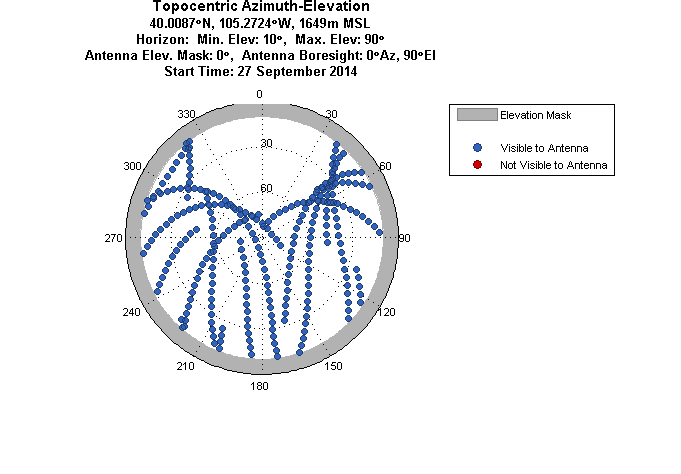
\includegraphics[height=2in]{Figures/PRN_Vis_201409271300MDT_6hr_Sidera}
	\end{subfigure}
	\begin{subfigure}
	\centering
 		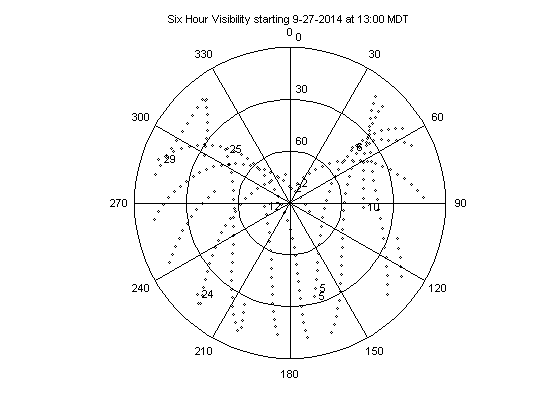
\includegraphics[height=2in]{Figures/PRN_Vis_201409271300MDT_6hr}
	\end{subfigure}
 	\caption{Left to right: Sidera output, computed output.}
 	\label{fig:SideraVsMe}
 \end{figure}

Satellites visible on September 27 at 1PM MDT were calculated from the YUMA almanac; the results are in Table ~\ref{PRNAzEl}.  Receiver data is shown in Figure ~\ref{fig:Receiver_sept271300}, qualitatively verifying the prediction.

\begin{table}[tbh]
\centering

\begin{tabular}{|c|c|c|}  
\hline
PRN & Azimuth & Elevation\\
\hline\hline
2 & $6.15^{\circ}$ & $81.65^{\circ}$\\  
\hline
5 & $165.20^{\circ}$ & $33.88^{\circ}$\\
\hline
6 & $48.57^{\circ}$ & $41.72^{\circ}$\\
\hline
10 & $93.49^{\circ}$ & $47.20^{\circ}$\\
\hline
12 & $-97.24^{\circ}$ & $75.14^{\circ}$\\
\hline
17 & $95.80^{\circ}$ & $8.09^{\circ}$\\
\hline
24 & $-134.77^{\circ}$ & $14.42^{\circ}$\\
\hline
25 & $-50.16^{\circ}$ & $41.43^{\circ}$\\
\hline
29 & $-71.73^{\circ}$ & $10.05^{\circ}$\\
\hline
\end{tabular}

\caption{PRN Azimuth/Elevation on September 27, 2014 at 1PM MDT}
\label{PRNAzEl}
\end{table}

 \begin{figure}[H]
 	\centering
 	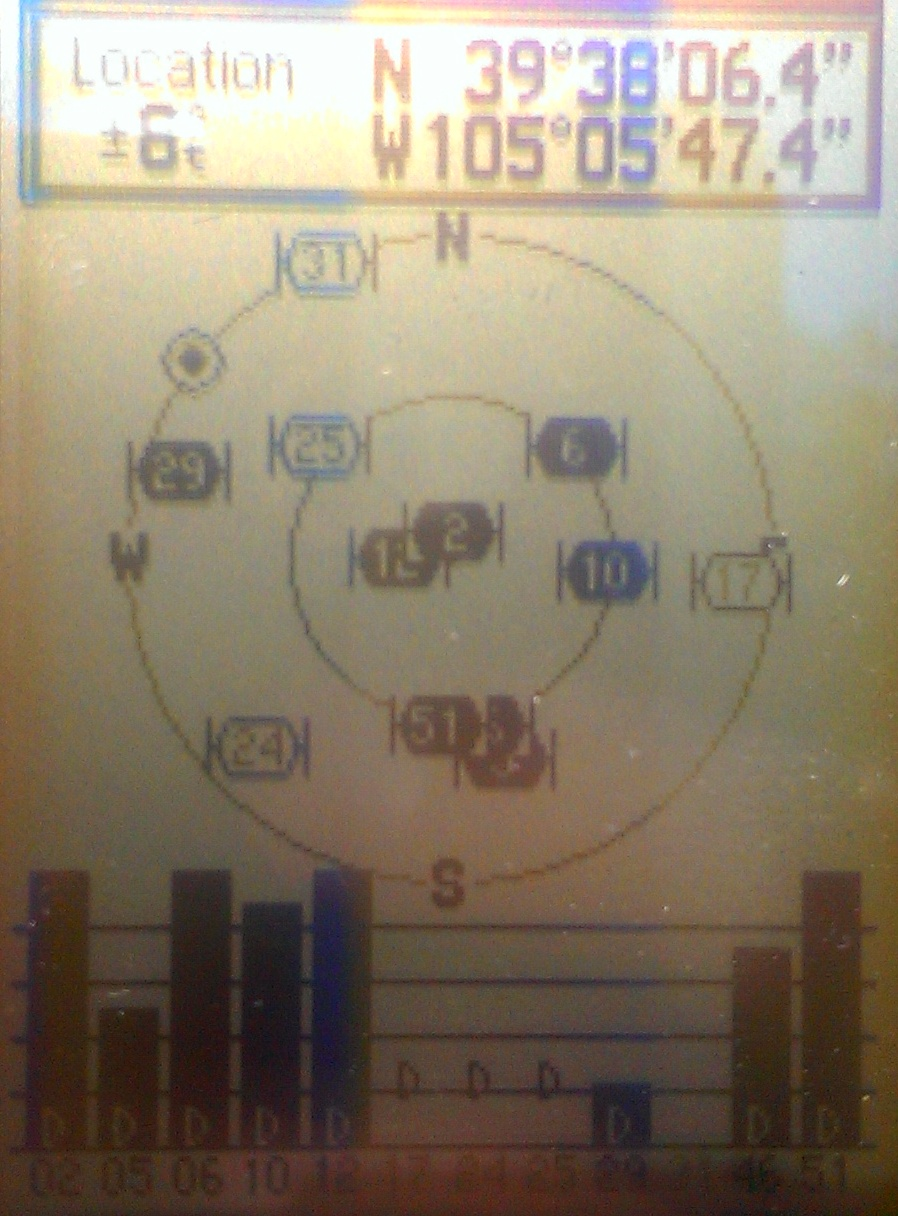
\includegraphics[height=2in]{Figures/sept271300}
 	\caption{Satellites visible to receiver on September 27, 2014 at 1PM MDT.}
 	\label{fig:Receiver_sept271300}
 \end{figure}

\pagebreak
\section{GPS Satellite Visibility}
To see daily coverage of multiple points on the earth, the ephemerides were propagated for a day.  Locations were chosen to be at the North pole, the equator, and Boulder, CO.  The azimuth/elevation plots are shows in Figure ~\ref{fig:3Coverage}.


\begin{figure}[H]
 	\centering
	\begin{subfigure}
	\centering
 		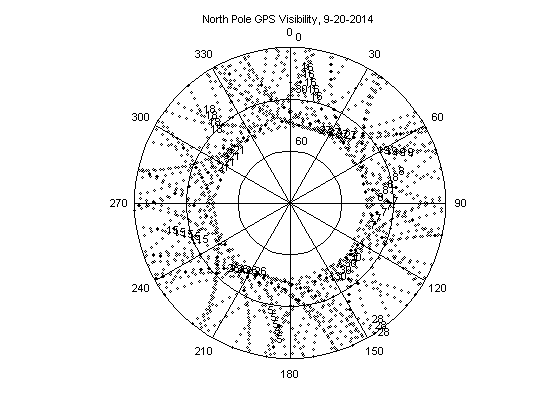
\includegraphics[height=2in]{Figures/PRN_Vis_NP_201409200000MDT_24hr}
	\end{subfigure}
	\begin{subfigure}
	\centering
 		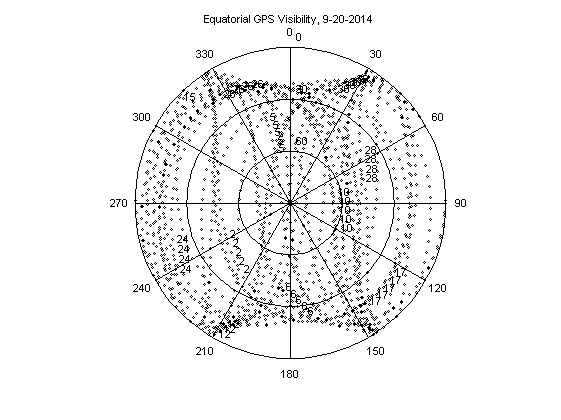
\includegraphics[height=2in]{Figures/PRN_Vis_Equator_201409200000MDT_24hr}
	\end{subfigure}
	\begin{subfigure}
	\centering
 		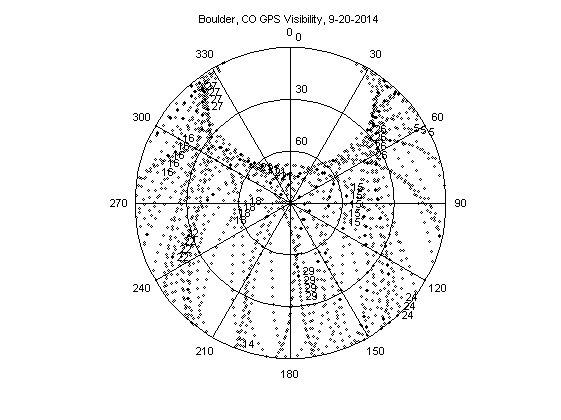
\includegraphics[height=2in]{Figures/PRN_Vis_Boulder_201409200000MDT_24hr}
	\end{subfigure}
 	\caption{GPS satellite visibility from different points on the earth.}
 	\label{fig:3Coverage}
 \end{figure}

The equatorial plot shows two holes: one to the north and one to the south. This result makes sense, as the GPS satellites have inclinations of approximately $55^{\circ}$.  That limits the elevation to the north and the south that satellites can be seen.  Boulder, 40 degrees north of the equator, shows a hole to the north for the same reason; there is no hole in visibility to the south due to the latitude of the location and the satellite inclination.  At the North pole, the hole is directly above the point.  This hole again is a result of the satellite inclinations, which are not polar.  The maximum elevation for the North pole case is demonstrated in Figure ~\ref{fig:Pole}. 

\begin{figure}[H]
 	\centering
 	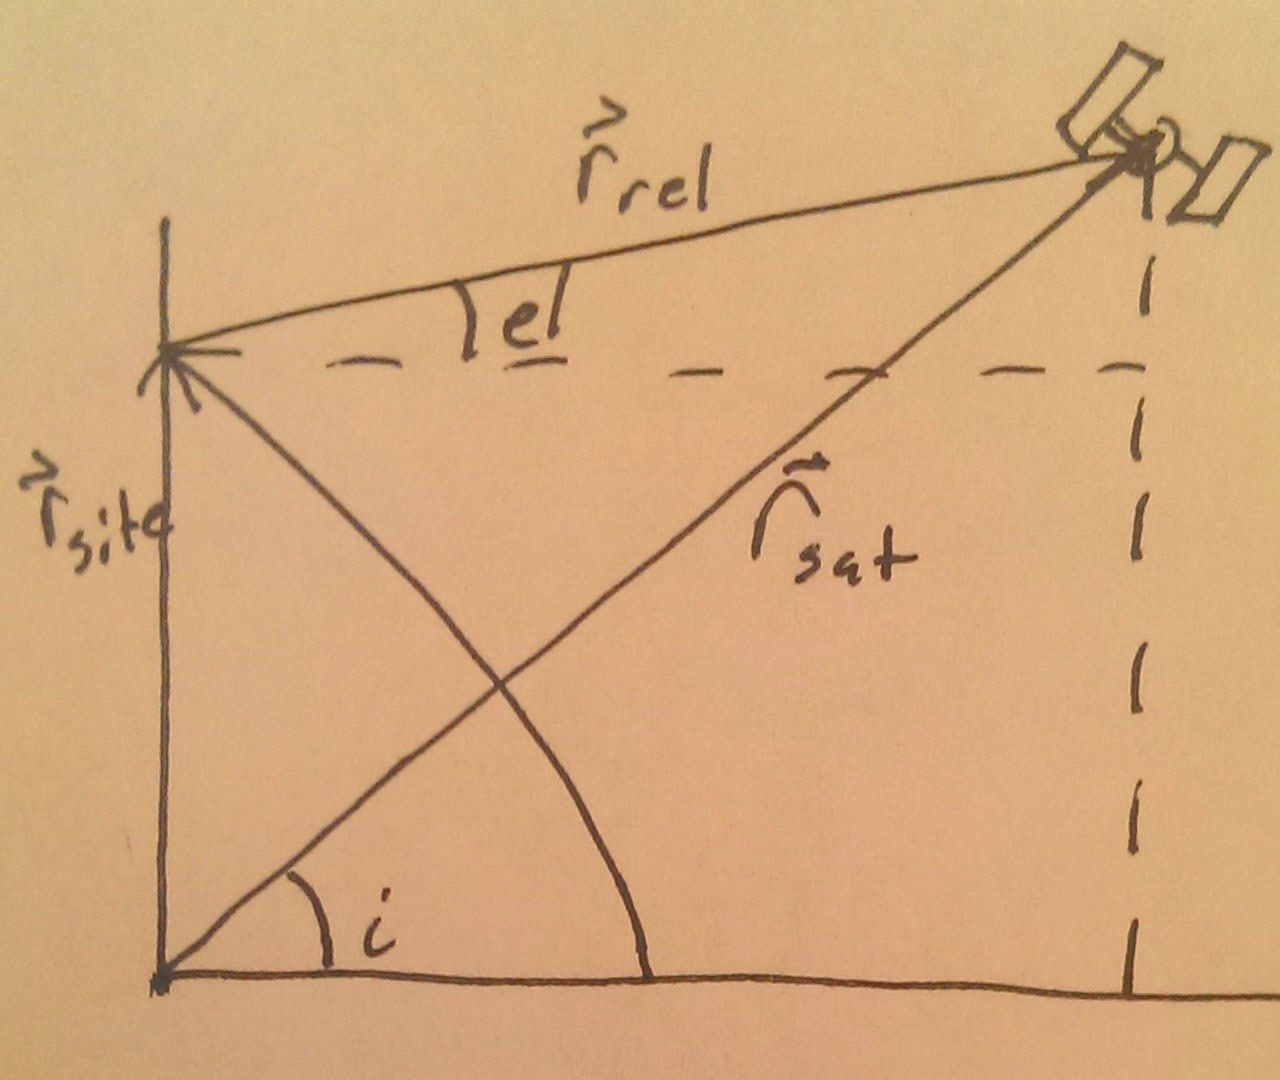
\includegraphics[height=2in]{Figures/pole}
 	\caption{Planar view of satellite at its highest latitude being viewed from the North Pole.}
 	\label{fig:Pole}
 \end{figure}

The maximum elevation be roughly analytically calculated as
\begin{equation}\label{eq:NP_Max_El}  
el=\arctan \left ( \frac{r_{sat}\sin i-r_{Earth}}{r_{sat}\cos i} \right )
\end{equation}
where $r_{sat}=26,600\textup{km}$, $i=55^{\circ}$, and $r_{Earth}=6378\textup{km}$.  The result of Equation ~\ref{eq:NP_Max_El} is a maximum elevation of approximately $45^{\circ}$.

The number of satellites visible from Boulder on September 27, 2014 are shown in Figure ~\ref{fig:numVisBoulder}. The results are shown for 24 hours.

\begin{figure}[H]
 	\centering
 	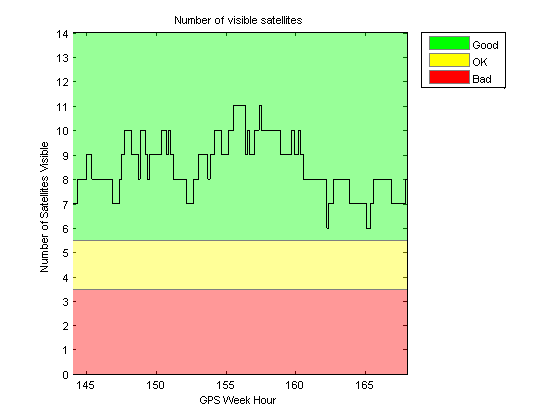
\includegraphics[height=2in]{Figures/num_sats_visible}
 	\caption{Number of visible satellites from Boulder, CO over 24 hours.}
 	\label{fig:numVisBoulder}
 \end{figure}

For a satellite to be visible in the same point in the sky on two consecutive days, the satellite period multiplied by an integer number of orbits must be a sidereal day (86164 seconds)\cite{MisraEnge}.  The orbit plane is essentially inertially fixed over the course of two days, and the change in other orbital elements are assumed to be negligible except for the true anomaly angle (although it must be the same as it previously was).  To determine how many orbits a satellite must complete to satisfy this requirement, 
\begin{equation}\label{eq:NP_Max_El}  
n = \textup{sidereal}/P
\end{equation}

where $n$ must be an integer.  It takes two orbits for GPS satellites to be in the same position in the sky one sidereal day later.  This is simulation results are shown in Table ~\ref{PRNAzElDiff} for selected PRNs.

\begin{table}[H]
\centering

\begin{tabular}{|c|c|c|}  
\hline
PRN & $\Delta$Azimuth & $\Delta$Elevation\\
\hline\hline
2 & $0.31^{\circ}$ & $-0.06^{\circ}$\\  
\hline
5 & $-0.02^{\circ}$ & $0.07^{\circ}$\\
\hline
6 & $0.03^{\circ}$ & $-0.10^{\circ}$\\
\hline
\end{tabular}

\caption[font=small,labelfont=bf]{PRN Azimuth/Elevation differences between 9/27/2014 19:00 UTC and 9/28/2014 18:56:4 UTC}
\label{PRNAzElDiff}
\end{table}

\section{Conclusions and Recommendations}
GPS satellite visibility for an observation site is latitude-dependent due to the satellite inclination.  The number of satellites and the spacing of the constellation's orbit planes ensures multiple satellites should be visible from any point on Earth (notwithstanding topography).  Each satellite was found to also occupy the same area in the sky one sidereal day later.  Visibility computations were qualitatively compared to proprietary code and looked accurate.  Unfortunately there was no known way to get computed satellite azimuth/elevation data from the receiver itself, so the comparisons had to be eyeballed (a potential error source in higher-fidelity research). Future investigations should look into the satellite-visibility geometry, based on computed visibility, and its connection to the accuracy of a receiver's measurement. 

\bibliographystyle{aiaa}   % Number the references.
\bibliography{ASEN5010ProjectBib}   % Use references.bib to resolve the labels.


\end{document}

